\documentclass[11pt]{article}
\usepackage[margin=1in]{geometry}
\usepackage{graphicx}
\usepackage{amsmath}
\usepackage{float}
\usepackage{setspace}
\setstretch{1.05}
\title{Internal Meta-Analysis of the Water Scarcity--GDP Growth Estimate}
\author{Draft for ECN 726 term project}
\date{\today}
\begin{document}
\maketitle
\begin{abstract}
This draft revisits the headline GDP-growth estimate in Frost, Madeira, and Martinez Jaramillo (2025) by running an internal meta-analysis over 120 alternative specifications. The replicated baseline coefficient on freshwater withdrawal as a share of available freshwater is -0.102 with standard error 0.039 on 4,583 observations. Across the specification set, the estimate distribution remains mostly negative, with a mean of -0.129 and a median of -0.131. The meta-regression shows that nonlinear forms and lower-tail quantile specifications make the scarcity effect substantially more negative, while random-effects and between estimators attenuate it.
\end{abstract}
\section{Introduction}
Frost, Madeira, and Martinez Jaramillo (2025) ask whether water scarcity has macroeconomically relevant effects on output, investment, and inflation. My focal metric is the coefficient on freshwater withdrawal as a share of available freshwater in the GDP growth regression reported in their Table 3, column (3). Using the replicated Stata workflow, I exactly reproduce that benchmark in the 1990--2020 panel used for the extension: the coefficient is -0.102 with standard error 0.039, N = 4,583, and R-squared = 0.219.
The extension treats this coefficient as one draw from a broader model space. Following Banzhaf and Smith (2007), I vary two dimensions of modeling choice: the functional form for scarcity and the panel estimator. The resulting 120 estimates are summarized with a specification curve and an auxiliary meta-regression. This design makes it possible to ask whether the negative scarcity--growth relationship is robust to economically motivated nonlinearities and to alternative ways of using within-country and between-country variation.
\section{Data}
The extension reuses the replication package data pipeline and merges the same four formatted panel sources used in the original GDP growth regressions: World Bank macro data, Aquastat water data, Worldwide Governance Indicators, and Penn World Table series. The merged panel is unbalanced and spans 169 countries over 1990--2020 after the extension's analysis-window check. The dependent variable is annual GDP growth. The baseline controls are log total water withdrawal per capita and log GDP per capita in PPP terms.
Water scarcity is measured three ways: freshwater withdrawal as a share of internal renewable resources, as a share of total renewable resources, and as a share of available freshwater. Consistent with the original code and the paper's description, each scarcity measure is capped at 100 and then carried into the regression pipeline after top-percentile winsorization. The panel retains the original sample differences across scarcity measures, so the internal-resource sample is slightly smaller than the renewable-resource and available-freshwater samples.
\section{Model Specification}
The original paper motivates the empirical analysis with a Cobb-Douglas production function in which water enters as an additional input and scarcity lowers effective productivity. Let output depend on TFP, capital, labor, and a scarcity-adjusted water term. Under the paper's parameterization, higher water scarcity lowers the productivity contribution of water through a factor proportional to $1/(1+WS_{ct})$. The empirical specification replaces the structural object with a linear panel-data approximation in which GDP growth is regressed on a scarcity measure, log water withdrawal per capita, log GDP per capita, country fixed effects, and year fixed effects.
This identifying strategy is informative but not causal. Reverse causality remains possible if weak growth reduces water demand or changes sectoral composition in ways that feed back into measured scarcity. Omitted variables are also a concern: institutions, trade exposure, energy composition, and sectoral structure may jointly shape both macro performance and water use. The extension therefore treats the focal estimate as an association whose stability can still be evaluated across plausible modeling choices, even though those choices do not solve endogeneity on their own.
\section{Analysis Design}
The first modeling dimension is functional form. The linear baseline preserves the authors' original design. A quadratic term tests whether the drag from scarcity steepens as water constraints tighten. An interaction with log GDP per capita asks whether richer countries buffer scarcity through infrastructure, technology, or sectoral composition. An interaction with log water use per capita tests whether high scarcity becomes more harmful when absolute water demand is also high. Finally, a threshold specification allows the scarcity slope to change above the median scarcity level, capturing the possibility that water becomes a binding constraint only after a critical point is reached.
The second dimension is estimator choice. Country fixed effects without year effects test whether global shocks matter for the baseline coefficient. Two-way fixed effects are the benchmark. Random effects and the Hausman comparison assess whether between-country variation carries useful information or is contaminated by omitted heterogeneity. The between estimator isolates long-run cross-country differences. First differences offer an alternative transformation that removes country effects through changes rather than demeaning. Machado and Santos Silva's (2019) panel quantile estimator is used at the 25th, 50th, and 75th percentiles without year fixed effects, in line with the authors' own ancillary-parameter caveat.
The meta-regression summarizes the estimate distribution as
\[
\begin{aligned}
\hat{\beta}_s =\ & \gamma_0 + \gamma_1 d_{quadratic,s} + \gamma_2 d_{income,s} + \gamma_3 d_{use,s} + \gamma_4 d_{threshold,s} + \gamma_5 d_{internal,s} + \gamma_6 d_{renewable,s} \\
& + \gamma_7 d_{countryFE,s} + \gamma_8 d_{RE,s} + \gamma_9 d_{between,s} + \gamma_{10} d_{FD,s} + \gamma_{11} d_{Q25,s} + \gamma_{12} d_{Q50,s} + \gamma_{13} d_{Q75,s} + \varepsilon_s,
\end{aligned}
\]
where the omitted categories are the linear form, the available-freshwater scarcity measure, and the two-way fixed-effects estimator.
\section{Analysis Results}
All 120 planned specifications converged, so the internal meta-analysis covers the complete design space. Table~\ref{tab:dist} reports the distribution of the resulting scarcity coefficients, and Table~\ref{tab:meta_ame} reports the AME-based meta-regression coefficients. The average estimate is -0.129, the median is -0.131, the interquartile range runs from -0.187 to -0.025, 84.2\% of the estimates are negative, and 39.2\% are statistically significant at the 5\% level. These moments already suggest that the sign of the relationship is usually stable even when the magnitude is not.
\begin{figure}[H]
\centering
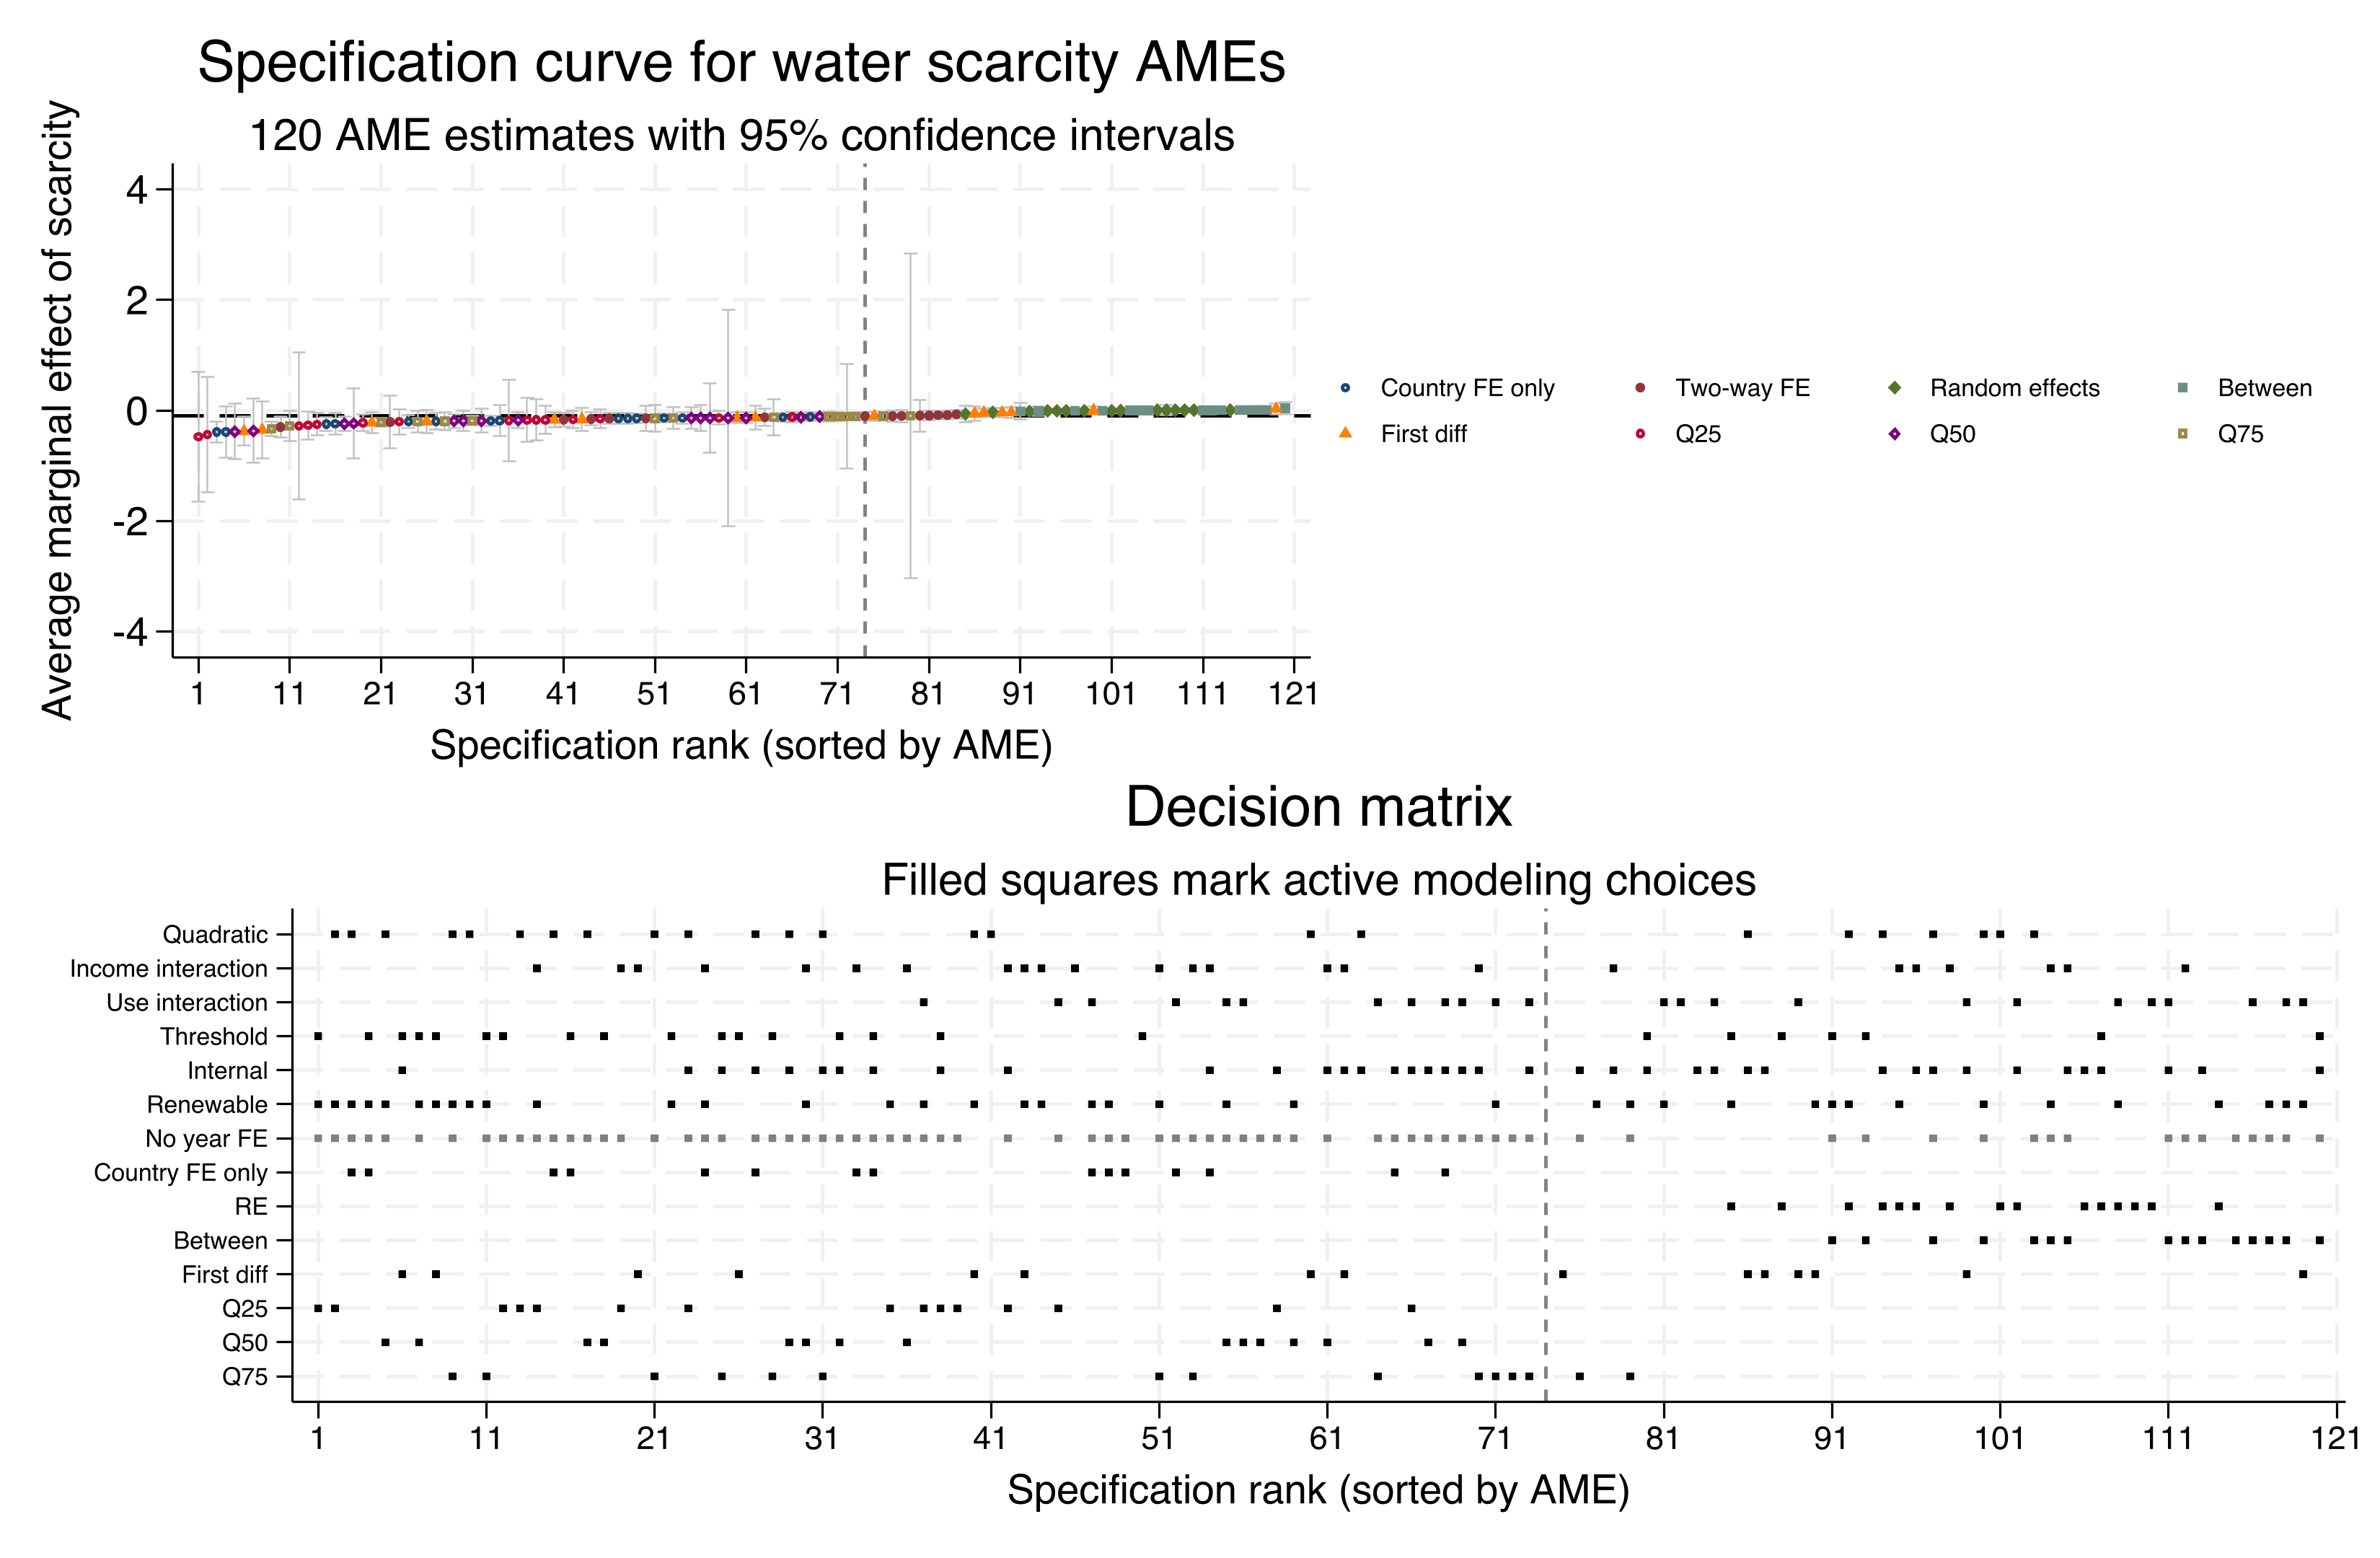
\includegraphics[width=\textwidth]{../figures/specification_curve.png}
\caption{Specification curve for the 120 water scarcity estimates}
\label{fig:spec_curve}
\end{figure}
\begin{table}[htbp]
\centering
\caption{Distribution of the 120 scarcity estimates}
\label{tab:dist}
\small
\begin{tabular}{lc}
\hline
Statistic & Value \\\\
\hline
Successful specifications & 120 \\\\
Mean beta & -0.292 \\\\
Median beta & -0.144 \\\\
25th percentile & -0.364 \\\\
75th percentile & -0.035 \\\\
Share negative (\%) & 85.8 \\\\
Share significant at 5\% (\%) & 29.2 \\\\
\hline
\end{tabular}
\end{table}

\begin{table}[htbp]
\centering
\caption{AME-based meta-regression of water scarcity estimates}
\label{tab:meta_ame}
\small
\begin{tabular}{lcc}
\toprule
Variable & Coefficient & Robust SE \\\\
\midrule
Constant & -0.0793 & 0.0138 \\\\
Quadratic form & -0.0939 & 0.0152 \\\\
Scarcity x log GDP per capita & -0.0396 & 0.0102 \\\\
Scarcity x log water use & 0.0093 & 0.0125 \\\\
Threshold form & -0.1102 & 0.0182 \\\\
Internal scarcity measure & 0.0269 & 0.0103 \\\\
Renewable scarcity measure & -0.0368 & 0.0122 \\\\
No year fixed effects & -0.0675 & 0.0155 \\\\
Random effects & 0.1221 & 0.0157 \\\\
Between estimator & 0.2015 & 0.0185 \\\\
First differences & -0.0011 & 0.0259 \\\\
Quantile 0.25 & -0.0277 & 0.0200 \\\\
Quantile 0.50 & 0.0073 & 0.0161 \\\\
Quantile 0.75 & 0.0354 & 0.0152 \\\\
\bottomrule
\multicolumn{3}{p{0.9\textwidth}}{\footnotesize Notes: OLS meta-regression with heteroskedasticity-robust standard errors. The dependent variable is the specification-level average marginal effect (AME) of water scarcity on GDP growth. The omitted categories are the linear functional form, the available-freshwater scarcity measure, and the two-way fixed-effects estimator. The no-year-fixed-effects dummy captures the country-FE-only shift relative to the two-way FE baseline, while the between and quantile coefficients are incremental deviations on top of that no-year-FE penalty.}
\end{tabular}
\end{table}

Figure~\ref{fig:spec_curve} shows that the authors' baseline estimate lies in the middle of a much wider but still mostly negative distribution. The meta-regression indicates that several modeling choices systematically shift the estimate away from the baseline.
Relative to the two-way fixed-effects linear baseline, the quadratic specification lowers the coefficient by -0.094 (p=0.000), the income interaction lowers it by -0.040 (p=0.000), and the threshold model lowers it by -0.110 (p=0.000). These are economically meaningful changes: each one makes the scarcity effect substantially more negative.
Estimator choice also matters. In the AME meta-regression, the no-year-FE dummy is negative (-0.068, p=0.000), which means that the country-FE-only specification is more negative than the two-way fixed-effects baseline once the functional-form and scarcity-measure controls are held fixed. Random-effects and between estimators then shift the coefficient upward by 0.122 (p=0.000) and 0.202 (p=0.000) relative to their own reference cells. This pattern is consistent with the idea that the within-country signal is more negative than the between-country correlation, while models that omit year effects inherit an additional negative shift.
The quantile results reinforce the paper's tail-risk interpretation. The Q25 and Q50 coefficients are -0.028 and 0.007 below the baseline meta-regression constant, while the Q75 shift is 0.035 (p=0.021). Lower-tail growth episodes therefore appear especially sensitive to water scarcity.
\begin{figure}[H]
\centering
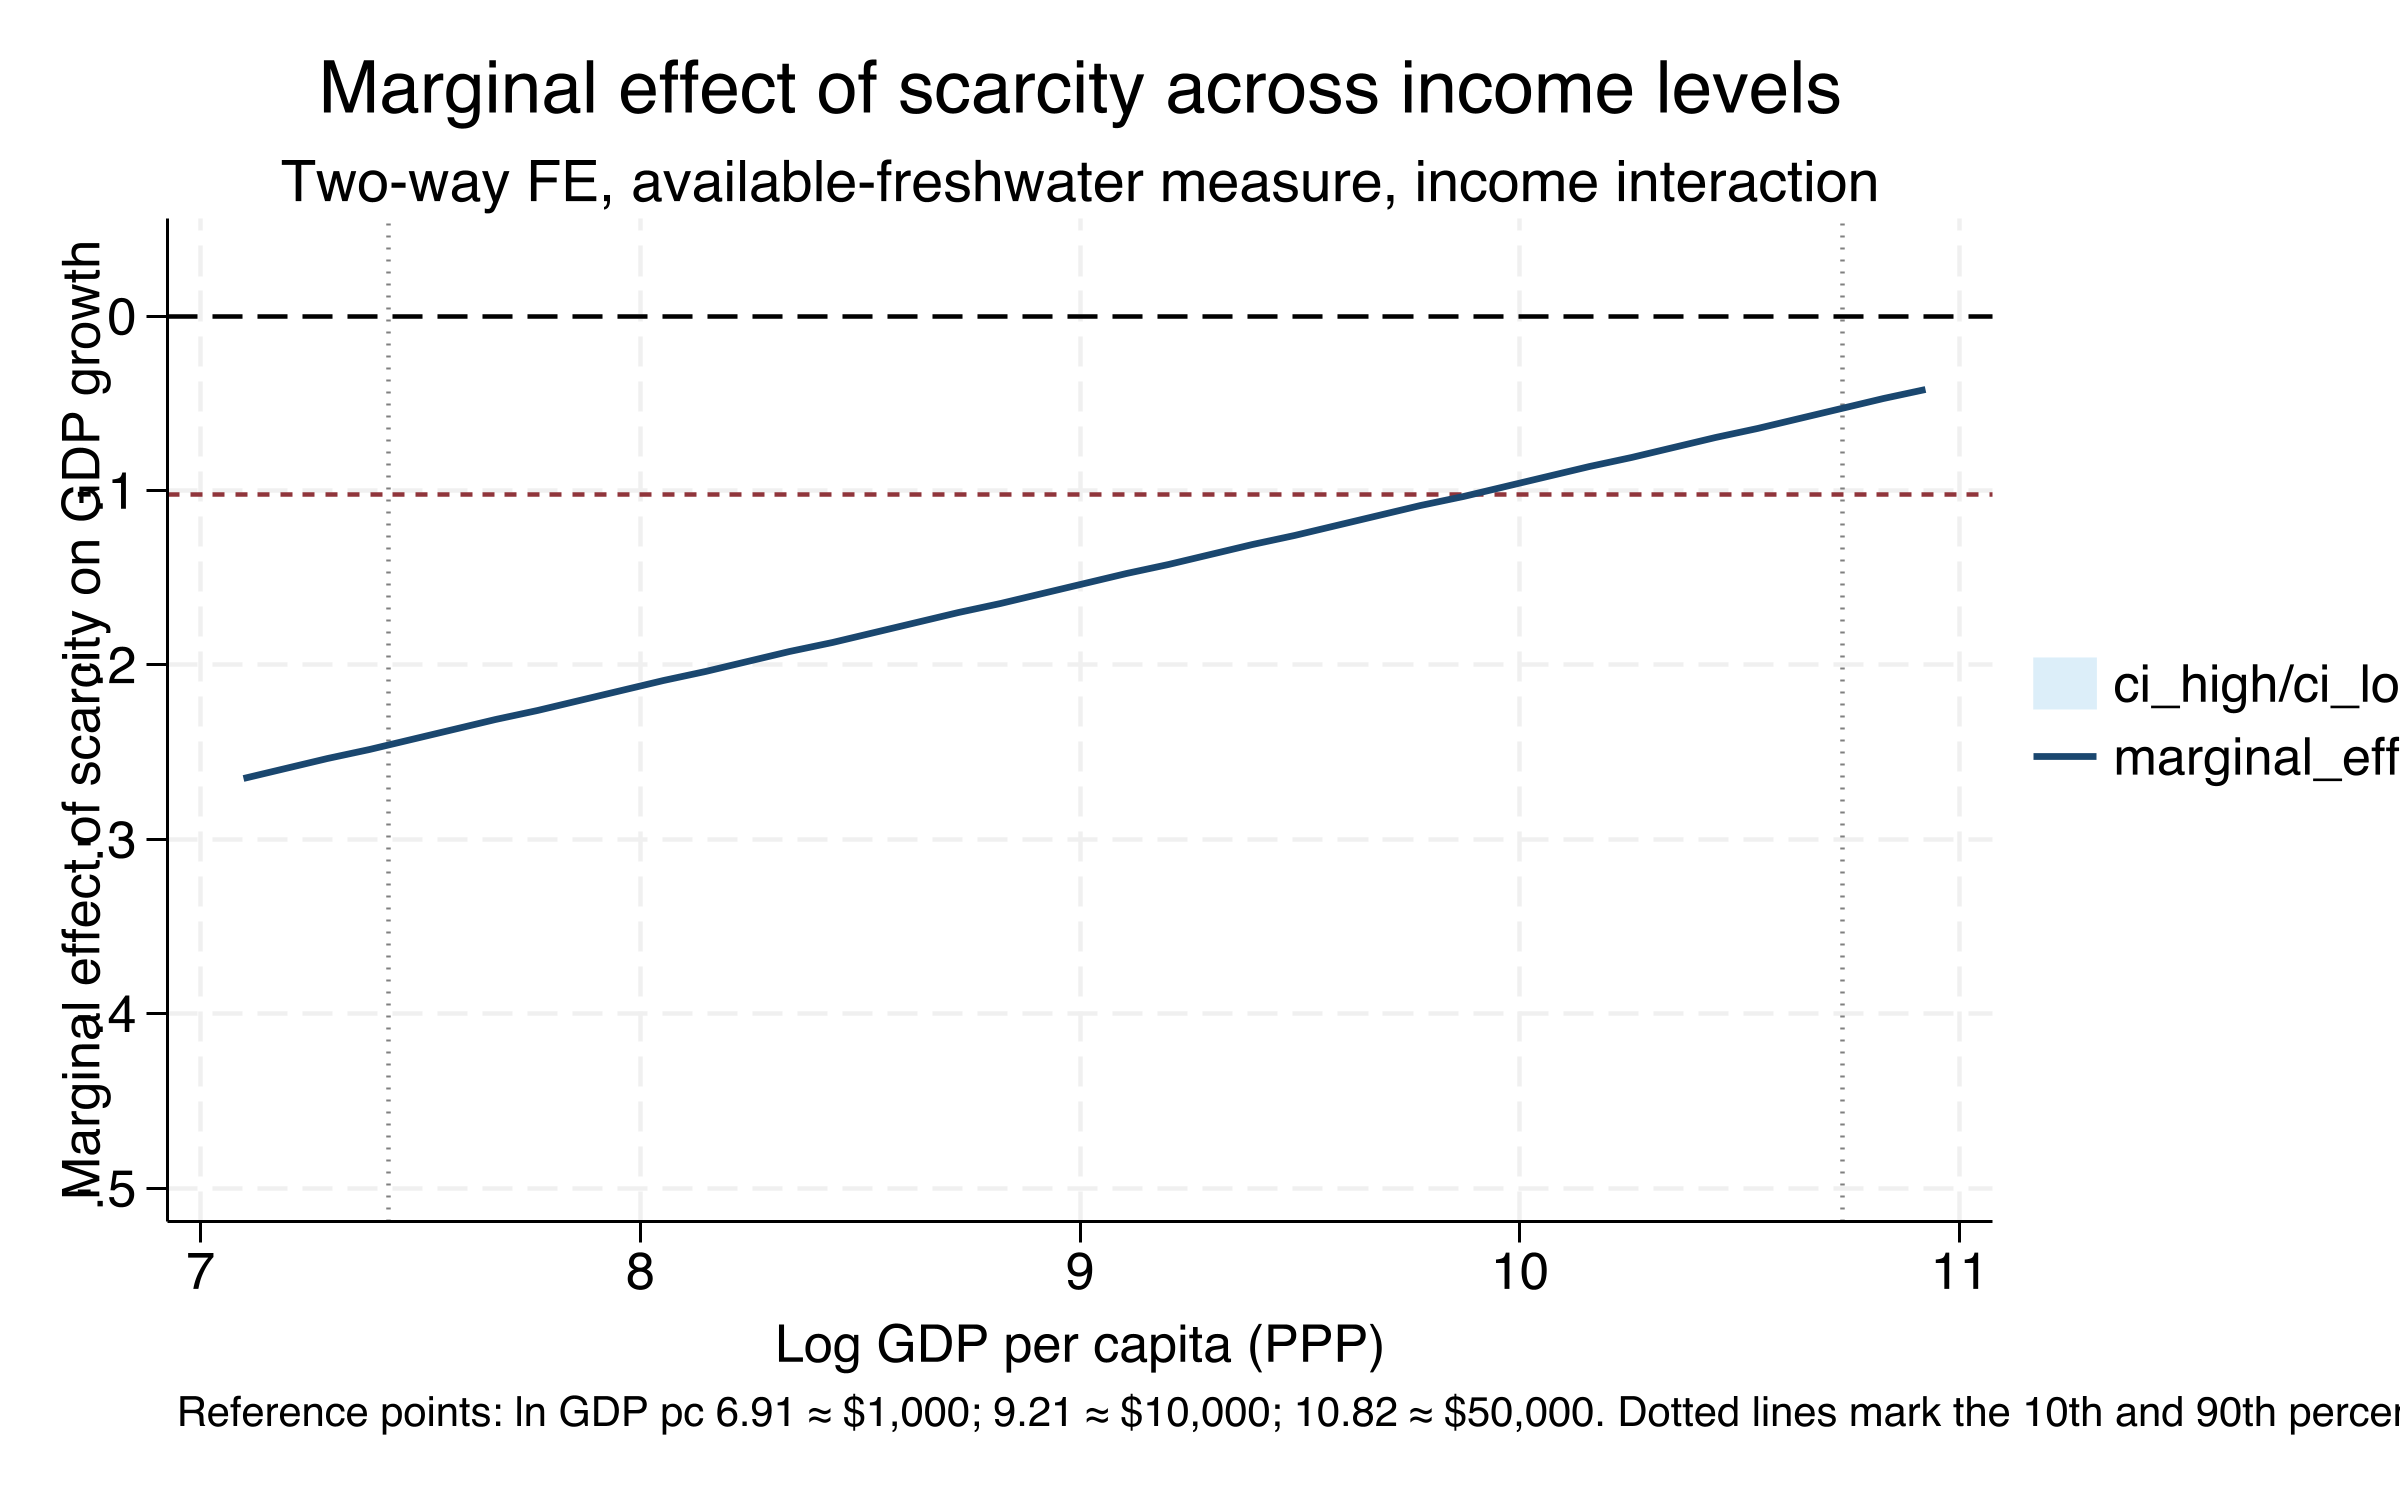
\includegraphics[width=0.85\textwidth]{../figures/marginal_effect_income.png}
\caption{Marginal effect of water scarcity across income levels}
\label{fig:marginal_income}
\end{figure}
Figure~\ref{fig:marginal_income} visualizes the two-way fixed-effects income-interaction specification for the available-freshwater measure. The point estimate becomes less negative as income rises, which is consistent with the idea that richer economies can partially buffer water constraints through infrastructure, technology, or sectoral composition. The confidence band approaches zero only near the upper end of the income distribution, so the attenuation is economically meaningful even though the sign does not reverse over most of the observed support.
\begin{figure}[H]
\centering
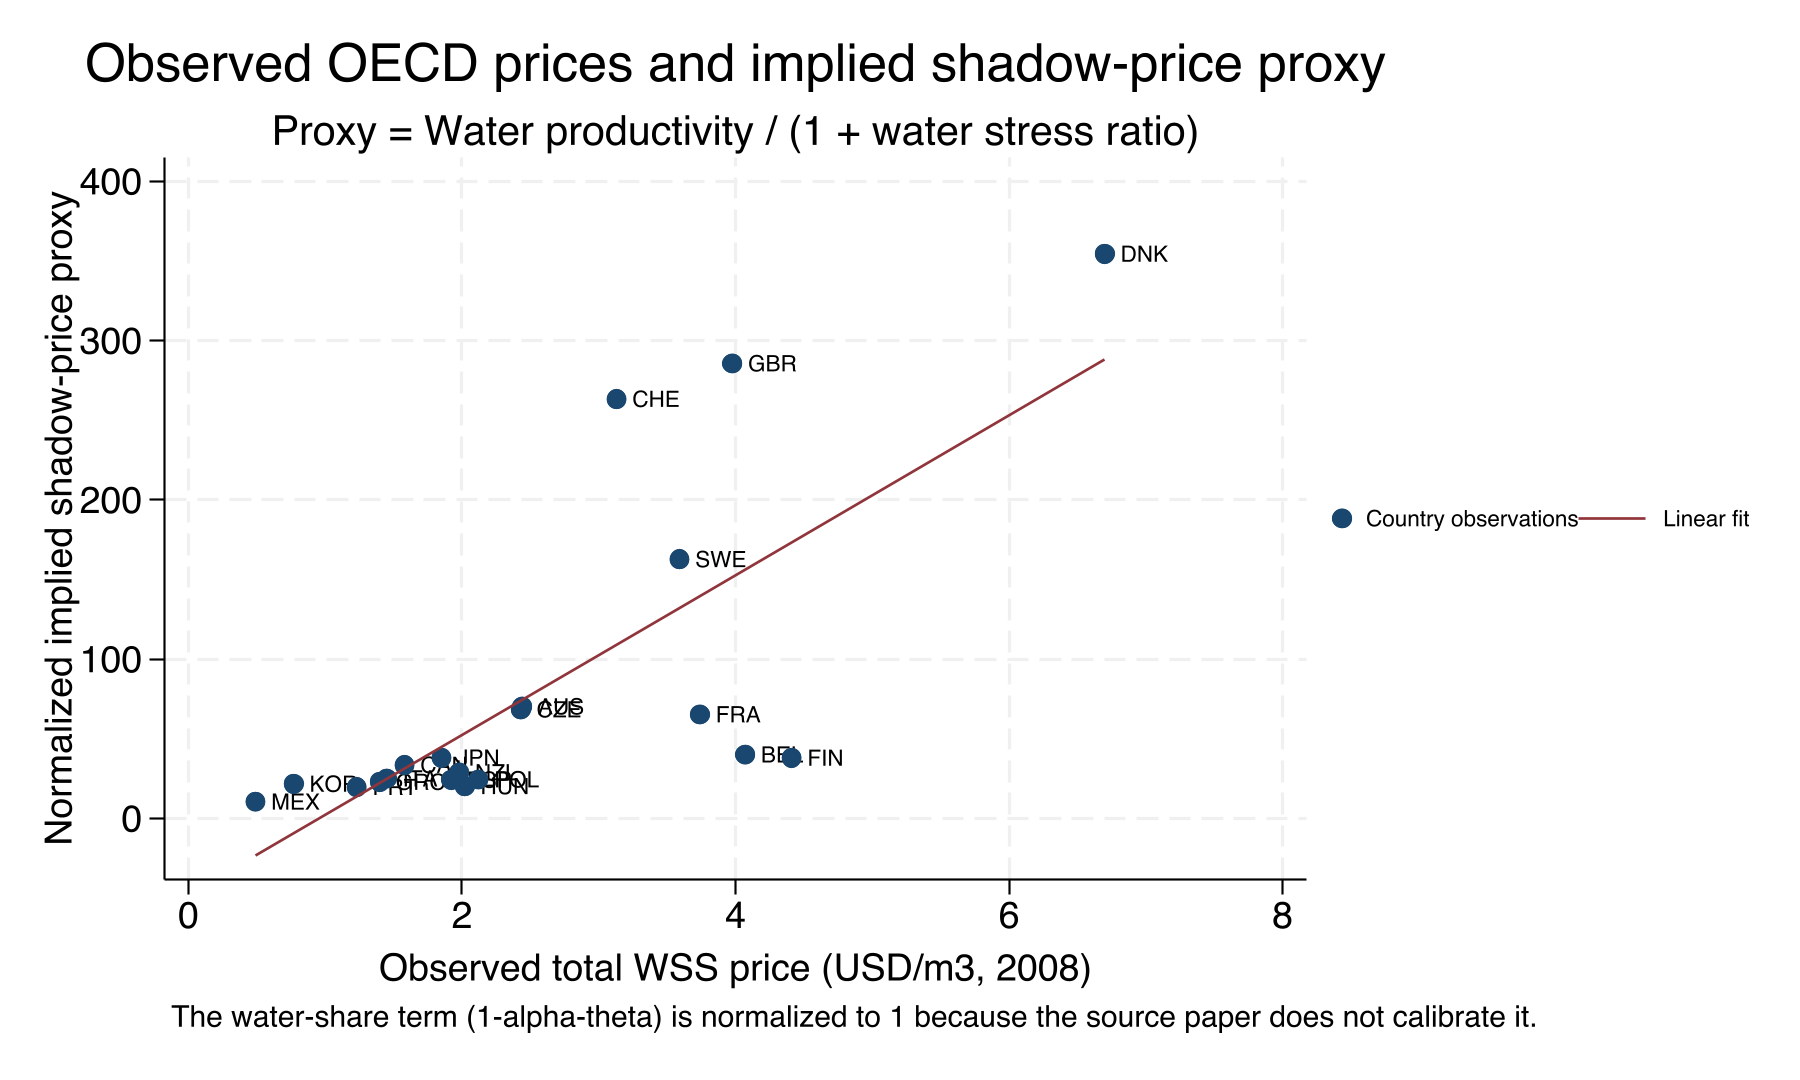
\includegraphics[width=0.9\textwidth]{../figures/shadow_price_proxy.png}
\caption{Observed OECD water prices and the normalized implied shadow-price proxy}
\label{fig:shadow_price}
\end{figure}
The supplementary pricing figure compares observed OECD water supply and sanitation prices with a normalized implied shadow-price proxy computed as water productivity divided by one plus the water-stress ratio. Because the source paper does not calibrate the water-share term in the Cobb-Douglas model, the figure normalizes that term to one. The figure should therefore be read as a cross-country pricing diagnostic rather than as a structural estimate of the level of the marginal product of water.
\section{Conclusions}
The extension supports the paper's central claim that water scarcity is associated with weaker macroeconomic performance. The sign of the scarcity coefficient is negative in most specifications, and the lower-tail quantile estimates are especially adverse. At the same time, the magnitude is not invariant. Functional forms that allow for nonlinear or heterogeneous effects tend to amplify the drag from scarcity, while estimators that rely more heavily on between-country variation attenuate it.
These results suggest that the original two-way fixed-effects estimate is informative but incomplete. Water scarcity appears to matter most in fragile growth states and in specifications that let scarcity interact with the level of development or with threshold effects. Future work should focus on richer controls for sectoral composition, trade, and institutions, and on designs that can better address reverse causality and omitted-variable bias. A more structural pricing exercise would also require an explicit calibration of water's production share rather than the normalization used here.
\begin{thebibliography}{9}
\bibitem{banzhaf_smith_2007} Banzhaf, H. Spencer, and V. Kerry Smith. 2007. Meta-analysis in model implementation: Choice sets and the valuation of air quality improvements. \textit{Journal of Applied Econometrics} 22(6): 1013--1031.
\bibitem{frost_madeira_mj_2025} Frost, Jon, Carlos Madeira, and Serafin Martinez Jaramillo. 2025. The economics of water scarcity. BIS Working Papers No. 1314.
\bibitem{machado_santos_silva_2019} Machado, Jose A. F., and J. M. C. Santos Silva. 2019. Quantiles via moments. \textit{Journal of Econometrics} 213(1): 145--173.
\bibitem{oecd_2010} OECD. 2010. \textit{Pricing Water Resources and Water and Sanitation Services}. Paris: Organisation for Economic Co-operation and Development.
\end{thebibliography}
\end{document}
